\chapter{Conclusion}
\label{chapter6}

%\setlength{\epigraphrule}{0pt}
\epigraph{\textit{If you can't fly then run, if you can't run then walk, if you can't walk then crawl, but whatever you do you have to keep moving forward.}}{ -- Martin Luther King Jr.}

% **************************** Define Graphics Path **************************
\ifpdf
    \graphicspath{{Chapter6/Figs/Raster/}{Chapter6/Figs/PDF/}{Chapter6/Figs/}}
\else
    \graphicspath{{Chapter6/Figs/Vector/}{Chapter6/Figs/}}
\fi

\section{Summary}

Recognizing complex event in videos has become an important task in computer vision due to various applications. However, this is a challenging task because we have to deal with real videos. In summary, there are four main challenges that we need to handle:
\begin{enumerate}
	\itemsep0em 
	\item \textit{Large content variation}.
	\item \textit{Uncontrolled capturing condition.}
	\item \textit{Large scale video dataset.}	
	\item \textit{Near-miss videos.}
\end{enumerate}
	
  The most important challenge that need to be handled is \textit{uncontrolled capturing condition}. This challenge of internet videos often harm the performance of event detection systems that was built on action recognition techniques. We handle this challenge by decomposing the original videos into segments and investigating \textit{feature representation}, \textit{feature aggregation}, and \textit{feature learning} methods from these segments. Beside this main challenge, we also deal with the \textit{large content variation} and \textit{large scale video dataset} as well. To this end, we made following contributions:

\begin{enumerate}
	\item We propose a new \textit{feature representation} method, named segment-based representation (\textbf{SB}), to overcome the limitations of the traditional video-based approaches. The basic idea is to examine shorter segments instead of using the representative frames or entire video. We carry thorough experiments to verify our proposed method by investigating different strategies to decompose a video into segments. These strategies include uniform segment sampling and segments based on shot boundary detection. By using more training examples (at segment level), this method can handle the \textit{large content variation} challenge as well.
	
	\item We propose a new \textit{feature aggregation} method, called sum-max video pooling (\textbf{SM}), to deal with noisy information in complex videos. This pooling technique is based on the layer structure of video. Basically, we apply sum pooling at the low layer representation while using max pooling at the high layer representation. Sum pooling is used to keep sufficient relevant features at the low layer, while max pooling is used to retrieve the most relevant features at the high layer, therefore it can discard irrelevant features in the final video representation. Our video pooling method is very efficient, thus it can be applied to \textit{large scale video dataset} as well.
	
	\item We propose a new \textit{feature learning} method, named Event-driven Multiple Instance Learning (\textbf{EDMIL}), to learn key evidences for complex event detection. We treat each segment as an instance and model it in a multiple instance learning framework \cite{andrews2002support}, where each video is a ``bag''. The instance-event similarity is quantized into different levels of relatedness. Intuitively, the most (ir)relevant instances should have higher (dis)similarities. Therefore, we propose to learn the instance labels by jointly optimizing the instance classifier and its related level. Similar to the first contribution, this method also use more training examples (at segment level), therefore it can handle the \textit{large content variation} challenge.
\end{enumerate}

It is beneficial to use some engineering tricks in order to handle large scale dataset. For example, the pre-computed kernel is suitable when there is a large number of events. In this case, we only need to calculate the kernel one time and train multiple time with different labels. This technique is especially useful in our EDMIL method.

A summary of the significant achievement of our proposed methods can be seen in Fig. \ref{c6_summary}. Our methods (SB, SM and EDMIL) can improve the baseline VideoBOW by \textbf{22.55 \%}, \textbf{2.67 \%} and \textbf{43.62 \%} respectively on the large scale MED 2011 dataset.

\begin{figure}
	\centering
	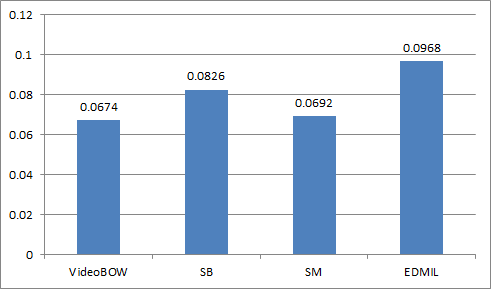
\includegraphics[width=0.9\textwidth]{summary.png}
	\caption{Performance comparison of our proposed solutions on the large scale MED 2011 dataset.}
	\label{c6_summary}
\end{figure}
	
\section{Future Work}
We plan to extend our work in following directions.
\begin{itemize}
	\item Learning the relationship between segments. Currently, we can learn a set of important segments that can be used for event detection. We have not imposed any constraints on the relation between segments. However, some spatial-temporal relationship might be important to identify an event. For example, in the event ``changing a vehicle tire'', the action ``removing hubcap'' should take place before the action ``replacing tire''. Or in the event ``flash mob gathering'', the ``gathering'' action should happen before the ``dancing'' action takes place. Moreover, some actions can have a co-occurrence relationship. For example, in the ``birthday party'' event, people can be both singing and dancing. 
	\item Learning the importance of each concept in the concept bank for event detection. Currently we only detect a set of concepts that can be used to provide evidences to detect an event. These concepts are obtained from NLP techniques. However, we do not know if it really visually represents for that event. It is interesting know which concepts that both textually and visually represent for an event.
\end{itemize}
